\chapter{Light Propagation in Linear Anisotropic Dielectrics}
\textit{"C'est mon chapitre préféré, celui que j'ai choisi lorsque j'étais à votre place. Ne ne négligez pas!}

\section{Anisotropic Materials in Photonics}
Beaucoup de matériaux ont des propriétés optiques quid épendent de la direction de la lumière ou de sa polarisation. 
Notons que dans un polariseur, si les polymères sont étendus en $y$, l'onde qui passera sera en $x$ !

\section{The Susceptibility and Dielectric Tensors}
\subsection{Constitutive Equations in Anisotropic Media}
	\begin{wrapfigure}[8]{l}{8cm}
	%\vspace{-5mm}
	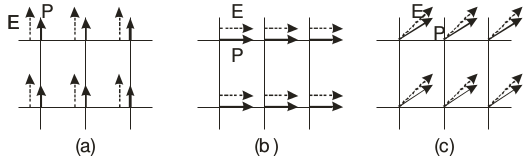
\includegraphics[scale=0.4]{ch4/image1.png}
	\captionof{figure}{ }
	\end{wrapfigure}
Lorsque le matériau n'est pas isotrope, $\vec{P}$ n'est pas toujours parallèle à $\vec{E}$ : la polarisation va
dépendre de la direction du champ électrique. Si dans une direction nous avons $n_1$ et dans une autre $n_2$ 
avec $n_a<n_b$, la superposition des deux donnera une polarisation non parallèle au champ appliqué. \\

La relation linéaire la plus générale entre deux vecteurs est un tenseur du second rang. Dès lors
\begin{equation}
P = \epsilon_0\overline{\overline{\chi}}E\qquad\text{ou}\qquad P_i = \epsilon_0\chi_{ij}E_j
\end{equation}
où $\overline{\overline{\chi}}$ est le \textbf{tenseur de susceptibilité}. S'il est diagonal avec tout des 
coefficients identiques, on se retrouve au cas du chapitre 2. Mais si non, la polarisation induite peut dépendre
de la direction de $\vec{E}$.

\subsection{Symmetry of the Susceptibility Tensor}
Il est simple de montrer analytiquement que le tenseur de susceptibilité est symétrique (sous certaines conditions).
Soit le théorème de Poynting
\begin{equation}
\dfrac{\partial U}{\partial t} = -\nabla.S-EJ_p
\end{equation}
où $U$ est la densité d'énergie EM et $\vec{S}$ le vecteur de Poynting
\begin{equation}
U = \frac{1}{2}\epsilon_0\left(|E|^2-c^2|B|^2\right),\qquad\qquad
S \equiv \left\langle \vec{E}\times\vec{H}\right\rangle = \frac{1}{\mu_0}
\left\langle \vec{E}\times\vec{B}\right\rangle
\end{equation}
Comme il  n'y a pas de courants libre, de magnétisation, le milieu est transparent et non-dissipant, l'énergie
n'est pas convertie en chaleur. L'énergie du champ peut aller dans la matière, mais elle sera "rendue" au final.
Il doit donc être possible de noter le troisième terme sous la forme d'une dérivée temporelle ou d'une divergence
afin de la faire passer dans le membre de gauche.\\

Dans la convention d'Einstein
\begin{equation}
E_kJ_{p,k} = E_k\frac{\partial P_k}{\partial t} = \frac{1}{2}E_k\epsilon_0\chi_{kl}\frac{\partial E_l}{\partial t}+
\frac{1}{2}E_l\epsilon_0\chi_{lk}\frac{\partial E_k}{\partial t}
\end{equation}
On peut toujours écrire $\chi_{kl} = \chi_{kl}^S+\chi_{kl}^A$. Il nous faudra montrer que $\chi_{kl}^A$ est
nulle. Le terme source devient\footnote{Voir page 62 pour le détail}
\begin{equation}
E_kJ_{p,k} = \frac{1}{2}\epsilon_0\chi_{kl}^S\frac{\partial (E_kE_l)}{\partial t}+\frac{1}{2}
\epsilon_0\chi_{kl}^A\left(E_k\frac{\partial E_l}{\partial t}-E_l\frac{\partial E_k}{\partial t}\right)
\end{equation}
Seule la partie symétrique peut s'écrire sous la forme d'une dérivée temporelle, la partie antisymétrique doit
forcément être nulle. Poynting s'écrit alors
\begin{equation}
\dfrac{\partial U_{total}}{\partial t}= -\nabla S
\end{equation}
où $U_{total}$ est la densité d'énergie totale
\begin{equation}
U_{total} = \frac{1}{2}D.E+\frac{1}{2}B.H
\end{equation}
Ceci n'est vrai que pour les matériaux non magnétique et non-dispersif.


\section{Plane Monochromatic Waves in Anisotropic Media}
\subsection{Dispersion Relation}
Nous allons ici analyser sir les ondes planes monochromatiques sont toujours solutions des équations de 
Maxwell et des équations constitutives (soit les équations de l’électrodynamique). Nous avons\footnote{Détails
page 63}
\begin{equation}
\nabla\times\left(\nabla\times\vec{E}\right) = -\frac{1}{c^2}\dfrac{\overline{\overline{\epsilon}}}{\epsilon_0}
\frac{\partial^2E}{\partial t^2}
\label{eq:4.41}
\end{equation}
C'est difficile, mais il existe un système de coordonnées ou ce tenseur est diagonal : tout va devenir "simple"
\footnote{Résultat attendu : le tenseur $\epsilon$ doit être symétrique, il doit exister une base où il est
diagonal}. Dans un tel système, le tenseur diélectrique est donné par (semble trivial, mais en réalité profond)
\begin{equation}
\dfrac{\overline{\overline{\epsilon}}}{\epsilon_0} =\left(\begin{array}{ccc}
n_1^2 & 0 &0\\
0 &n_2^2 &0\\
0&0&n_3^2
\end{array}\right)
\end{equation}
où $n_i$ sont les indices de réfraction principaux. L'équation \eqref{eq:4.41} devient quelque chose de 
"\textit{pas si moche}" : 
\begin{equation}
\vec\nabla\times(\vec\nabla\times\vec E) = -\frac{1}{c^2}\left(\vec{1_x} n_1^2\dfrac{\partial^2 E_x}{\partial t^2}
+\vec{1_y} n_2^2\dfrac{\partial^2 E_y}{\partial t^2}+\vec{1_z} n_3^2\dfrac{\partial^2 E_z}{\partial t^2}\right)
\end{equation}
On veut trouver une relation de dispersion $\omega(k)$. On propose une solution d'onde plane monochromatique 
de pulsation $\omega$ et de vecteur d'onde $\vec{k}$ à cette équation différentielle
\begin{equation}
E = E_0e^{i(\omega t-k.r)}
\end{equation}
En substituant cet ansat, on trouve (rot $\to\ ik$)
\begin{equation}
i\vec k\times(i\vec k\times \vec E_0) = \frac{\omega^2}{c^2}\left(\vec 1_x n_1^ 2 E_{0x}+
\vec 1_y n_2^ 2 E_{0y}+\vec 1_z n_3^ 2 E_{0z}\right)
\end{equation}
Sachant que $\vec A\times(\vec B\times \vec C) = -(\vec A\vec B)\vec C+(\vec A\vec C)\vec B$ 
\begin{equation}
\vec k(\vec k . \vec E_0) - \vec E_0 k^2 = -\frac{\omega^2}{c^2}\left(\vec 1_x n_1^ 2 E_{0x}+
\vec 1_y n_2^ 2 E_{0y}+\vec 1_z n_3^ 2 E_{0z}\right)
\label{eq:4.18}
\end{equation}
Il s'agit de la relation de dispersion pour un milieu linéaire non isentropique. En projetant cette équation 
sur les axes principaux (par exemple sur $\vec 1_x$ on a : $k_x \vec 1_x \left(k_x E_{0x} + k_y E_{0y} + k_z E_{0z}\right) - E_{0x} \vec 1_x\left(k_xk_x + k_y k_y + k_z k_z\right) =
-\frac{\omega^2}{c^2} \vec 1_x n_1^2 E_{0x}$) on voit que la relation de dispersion est un système linéaire
en les trois composantes du champ électrique\footnote{Savoir le faire avant de venir à l'examen.}
\begin{equation}
\left(\begin{array}{ccc}
\frac{\omega^2}{c^2}n_1^2-k_y^2k_z^2 & k_xk_y & k_xk_z\\
k_yk_x & \frac{\omega^2}{c^2}n_2^2-k_x^2-k_z^2 & k_yk_z\\
k_zk_x & k_zk_y & \frac{\omega^2}{c^2}n_3^2-k_x^2-k_y^2
\end{array}\right)\left(\begin{array}{c}
E_{0x}\\
E_{0y}\\
E_{0z}
\end{array}\right) = 0
\label{eq:4.19}
\end{equation}



\subsection{The Normal Surface}
Considérons d'abord quelques situations simplifiées. Avant tout, rappelons que la relation de dispersion
est la relation qui relie le comportement temporel au comportement spatial.
\begin{enumerate}
\item Vecteur d'onde parallèle à $\vec{1_x}$ : $k_x=k$. Le système \eqref{eq:4.19} se réduit à 
\begin{equation}
\left\{\begin{array}{rl}
\DS\frac{\omega^ 2}{c^2}n_1^2 E_{0x} &= 0\vspace{2mm}\\
\DS\left(\frac{\omega^2}{c^2}n_2^2-k^2\right)E_{0y}&=0\vspace{2mm}\\
\DS\left(\frac{\omega^2}{c^2}n_3^2-k^2\right)E_{0z}&=0
\end{array}\right.
\end{equation}
La première équation nous informe que le champ est transverse et les deux dernières les solutions : si l'un des $E_{0i}$ est non-nuls, la parenthèse doit l'être : on en tire la relations de dispersions tel que les deux 
autres composantes du champ sont nulles\footnote{C'est un système, il faut toujours préciser le triplet!}. La première est l'onde plane polarisée selon $y$ de nombre d'onde $k_2$
\begin{equation}
E^{(1)} = \vec{1_y}E_0^{(1)}e^{i(\omega t-k_2x)}\qquad\text{ où }\quad k_2 = \frac{\omega}{c}n_2
\end{equation}
La seconde est l'onde plane polarisée selon $z$ de nombre d'onde $k_3$
\begin{equation}
E^{(2)} = \vec{1_z}E_0^{(2)}e^{i(\omega t-k_3x)}\qquad\text{ où }\quad k_3 = \frac{\omega}{c}n_3
\end{equation}\ \\

\item Le vecteur d'onde $\vec k$ est dans le plan $xy$
\begin{equation}
\vec{1_k} = s_x\vec{1_x}+s_y\vec{1_y}
\end{equation}
Ce qui revient à substituer $k_z=0$ dans \eqref{eq:4.19}. A l'aide de la troisième équation du système,
on peut directement dire que $E_{0x}=E_{0y}$ et 
\begin{equation}
\vec E^{(1)} = \vec{1}_z E_0^{(1)}e^{i(\omega t-k_3\vec{1_k}.\vec{r}}\qquad\qquad
k_3=\dfrac{\omega}{c}n_3
\end{equation}
Il s'agit du mode propre de propagation, polarisé selon l'axe $z$, avec un nombre d'onde $k_3$. Notons que
cette solution ne tient pas compte de l'angle d'incidence. Les autres modes sont solutions de
\begin{equation}
\left(\begin{array}{cc}
\dfrac{\omega^2}{c^2}n^2_1-k_y^2 & k_xk_y\vspace{2mm}\\
k_yk_X&\dfrac{\omega^2}{c^2}n^2_2-k_x^2
\end{array}\right)\left(\begin{array}{c}
E_{0x}\\
E_{0y}
\end{array}\right) = 0
\end{equation}
Afin que ce soit vrai pour tout $E_{i0}$, le déterminant de ce système doit être singulier : cela donnera
les relations de dispersions
\begin{equation}
\left|\begin{array}{cc}
\dfrac{\omega^2}{c^2}n^2_1-k_y^2 & k_xk_y\vspace{2mm}\\
k_yk_X&\dfrac{\omega^2}{c^2}n^2_2-k_x^2
\end{array}\right|=0\qquad\Leftrightarrow\qquad \dfrac{k_x^2}{k^2_2}+\dfrac{k_y^2}{k^2_1}=1
\end{equation}
Il s'agit d'une ellipse avec comme axes $k_x$ et $k_y$ ! Attention à ne pas retenir cette formule sous
risque de se tromper : si on se propage selon $l_x$, la polarisation doit être selon $k_2$ (voila comment
le retenir).\\

\item \textbf{Cas général}. Pas le choix, il faut
résoudre
\begin{equation}
\left|\begin{array}{ccc}
\frac{\omega^2}{c^2}n_1^2-k_y^2k_z^2 & k_xk_y & k_xk_z\\
k_yk_x & \frac{\omega^2}{c^2}n_2^2-k_x^2-k_z^2 & k_yk_z\\
k_zk_x & k_zk_y & \frac{\omega^2}{c^2}n_3^2-k_x^2-k_y^2
\end{array}\right|=0
\end{equation}
Il s'agit de l'équation de la \textbf{surface normale}. En donnant la direction de propagation $\vec{1_k}$, il
y a en général deux intersections $\vec k=(k_x,k_y,k_z)$ entre cette direction et la surface normale. Celles-ci 
correspondent aux deux modes propres de propagation avec comme vitesse de phase $\omega/|\vec{k}|$. Une fois
la solution du vecteur d'onde connue, on peut trouver le mode propre de polarisation correspondant via
\eqref{eq:4.19}
\begin{equation}
\vec{E_0} = A_0\left(\dfrac{k_x}{k^2-k^2_1}\vec{1_x}+\dfrac{k_y}{k^2-k^2_2}\vec{1_y}+
\dfrac{k_z}{k^2-k^2_3}\vec{1_z}\right)
\end{equation}
Les trois composantes ayant la même phase, les modes propres sont donc linéairement polarisés. Si on 
calcule la solution du déterminant numériquement, on aura deux "coquilles" imbriquées. Essayons de 
retrouver ce résultat par analogie avec le résultat obtenu en 2., à savoir une ellipse. \\

Dans le plan $k_xk_y$ nous allons avoir une ellipse, mais également un cercle si la direction de propagation
est selon $\vec 1_z$ (ellipse dégénérée\footnote{Vérifier que c'est bien ça le sens.}). Si on "prolonge" ceci
dans le plan $k_zk_y$, l'ellipse va devenir un cercle ($n_x$, la direction de propagation) et le cercle une
ellipse ($n_z$). Enfin, dans $k_zk_x$ l'ellipse de $k_zk_y$ devient un cercle et l'autre une ellipse : il y
a un croisement. Avec de l'imagination, on retrouve le résultat présenté ci-dessous.
\begin{center}
	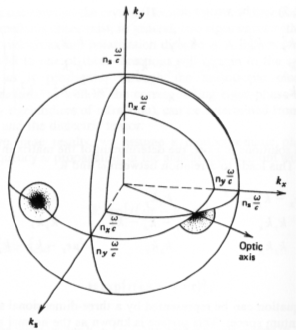
\includegraphics[scale=0.54]{ch4/image2.png}
	\captionof{figure}{ }
\end{center}

En général, les deux coquilles ont quatre points communs : ceux-ci définissent les \textbf{axes optiques}. En
ce point il n'y a qu'une solution : lorsqu'une onde se propage dans cette direction, sa vitesse de phase est
indépendantes de la polarisation. 
\end{enumerate}

\subsection{Fresnel’s Equation for the Dispersion Relation of Anisotropic Materials}
Nous venons de voir un première méthode de résolution, un peu lourde. Il en existe une seconde, plus simple,
mais jamais utilisée. La méthode se base sur une réécriture de la direction de propagation à l'aide des
cosinus directeurs
\begin{equation}
\vec k = \dfrac{\omega}{c}n\left(s_x\vec 1_x+s_y\vec 1_y+s_z\vec 1_z\right)
\end{equation}
où $n$ est la seule inconnue (!), l'indice de réfraction du milieu non-isotropique. On peut montrer 
("\textit{à essayer à la maison}") que l'on trouve
\begin{equation}
Dn^6+Cn^4+Bn^2+A=0
\end{equation}
Il s'agit d'une équation biquadratique, dont les solutions sont bien connues. Après quelque manipulations
de celles-ci on peut trouver
\begin{equation}
\dfrac{s^2_x}{n^2-n^2_1}+
\dfrac{s^2_y}{n^2-n^2_2}+
\dfrac{s^2_z}{n^2-n^2_3} = \dfrac{1}{n^2}
\end{equation}
Il s'agit de l'\textbf{équation de Fresnel} qui donne la relation entre les cosinus directeur, l'indice
$n$ que nous cherchons et les indices des directions. Malheureusement, on a ici perdu toutes les informations
sur la polarisation, heureusement que la troisième méthode est la ("\textbf{best method}"). Notons que cette
méthode est très instable numériquement. 

\subsection{The Index Ellipsoid}
Il s'agit de la troisième méthode, qui se base sur l'index ellipsoid. La méthode se base sur le champ de
déplacement $\vec{D}$ : celui-ci étant toujours transverse même dans les matériau anisotropique car 
$\div\vec{D} =0$. Nous allons alors utiliser la forme alternative de l'équation constitutive suivante
\begin{equation}
E_i = \dfrac{1}{\epsilon_0}\eta_{ij}D_j
\label{eq:4.34}
\end{equation}
où $\eta_{ij}$ est le tenseur d'imperméabilité adimensionnel. En combinant cette relation avec
$P_i = \epsilon_0\chi_{ij}E_j$, on trouve
\begin{equation}
\eta_{ij}\epsilon_{jk} = \epsilon_0\delta_{ik}
\end{equation}
La substitution de \eqref{eq:4.34} dans l'équation d'onde \eqref{eq:4.18} revient à 
\begin{equation}
\vec s\times\left(\vec{s}\times\overline{\overline{\eta}}.\vec{D}\right) = -\dfrac{1}{n^2}\vec{D}
\end{equation}
où $\vec{k}=n\vec{s}(\omega/c)$ avec $\vec{s}$ le vecteur unitaire dans la direction de propagation. 
Il s'agit de la relation de dispersion en fonction de $\vec{D}$. Le membre de droite (rot rot E) reste
le même mais le membre de droite devient simple. En supposant la propagation dans la direction $\vec{1_z}$,
on trouve en projetant dans le système de coordonnées 
\begin{equation}
\left(\begin{array}{ccc}
\eta_{11}&\eta_{12}&\eta_{13}\\
\eta_{21}&\eta_{22}&\eta_{23}
\end{array}\right)\left(\begin{array}{c}
D_x\\
D_y
\end{array}\right) = \dfrac{1}{n^2}\left(\begin{array}{c}
D_x\\
D_y
\end{array}\right)
\end{equation}
Le champ de déplacement est donc une solution du problème aux valeurs propres du la matrice 
d'imperméabilité transverse et on va pouvoir comprendre pourquoi on les appelle les modes propres de 
propagation. \\

Soit l'équation de l'\textbf{index ellipsoid}
\begin{equation}
\eta_{ij}\xi_i\xi_j=1
\end{equation}
où $\xi_i=D_i/(\sqrt{2\epsilon_0E.D})$ sont les coordonnées d'un espace abstrait. Dans les coordonnées
principales du système du tenseur diélectrique, l'index ellipsoid prend la forme
\begin{equation}
\dfrac{\xi^2_1}{n^2_1}+
\dfrac{\xi^2_2}{n^2_2}+
\dfrac{\xi^2_3}{n^2_3}=1
\end{equation}
Revenons à notre précédent système de coordonnées avec une propagation selon $\vec 1_z$. L'intersection
entre l'index ellipsoid et un plan perpendiculaire à la direction de propagation est une ellipse
\begin{equation}
\eta_{11}\xi^2_1 + 2\eta_{12}\xi_1\xi_2+\eta_{22}\xi_2^2=1
\end{equation}
Il en vient une procédure pour trouver les modes propre de propagation\footnote{Détail page 69.}
\begin{enumerate}
\item Trouver la direction de propagation
\item Considérer le plan perpendiculaire à la direction de propagation
\item Trouver l'intersection entre ce plan et l'ellipsoid index : l'intersection est une ellipse.
\end{enumerate}

A partir de cette ellispe résultant de l'intersection, on peut trouver deux choses
\begin{enumerate}
\item La direction des deux axes principaux de l'ellipse donne les directions de polarisation de $\vec{D}$
\item Les longueurs des axes principaux $d_1$ et $d_2$ permettent de trouver les indices de réfraction
\begin{equation}
n^{(1)} = \dfrac{d_1}{2}\qquad\qquad\qquad
n^{(2)} = \dfrac{d_2}{2}
\end{equation}
\end{enumerate}

Cette méthode est purement mathématique.






\subsection{Properties of the Eigenmodes of Propagation}
\subsubsection{Polarisation}
Le champ électrique du mode propre est donné par
\begin{equation}
\vec E = A_0\left(\dfrac{k_x}{k^ 2-k^2_1}\vec{1_x}+\dfrac{k_y}{k^ 2-k^2_2}\vec{1_y}+\dfrac{k_z}{k^ 2-k^3_1}\vec{1_z}
\right)
\end{equation}
Les phases de chaque composantes étant identiques, les modes propres sont polarisés linéairement.

\subsubsection{Orthogonal}
En générale $\vec{E}^{(1)}$ et $\vec{E}^{(2)}$ ne sont pas orthogonaux. Cependant, pour deux vecteurs propres
différents d'une matrice symétrique $\vec{D}^{(1)}$ et $\vec{D}^{(2)}$ le sont\footnote{Démo en exercice}.

\subsubsection{Transverse}
La première équation de Maxwell implique que le champ de déplacement de chaque mode propre est 
transverse (s'il n'y a pas de charges libres)
\begin{equation}
\vec\nabla.\vec{D} = 0\qquad\Leftrightarrow\qquad i\vec{k}.\vec{D} = 0\qquad\Leftrightarrow\qquad
\vec{s}.\vec{D} = 0
\end{equation}




\section{Energy Transport and Group Velocity}
\subsection{Properties of Poynting’s Vector}
On peut montrer que le flux de densité est donné par le vecteur de Poynting
\begin{equation}
\vec{S} = \vec{E}\times\vec{H}
\end{equation}
où $\vec{S}$ n'est en général pas colinéaire avec la direction de propagation. Considérons une onde EM 
constituée de la superposition de deux modes propres
\begin{equation}
\vec{E} = \alpha\vec{E}^{(1)}+\beta\vec{E}^{(2)}\qquad\qquad
\vec{H} = \alpha\vec{H}^{(1)}+\beta\vec{H}^{(2)}
\end{equation}
Le flux d'énergie est alors donné par
\begin{equation}
\begin{array}{ll}
\vec{S} &= \vec{E}\times\vec{H}\\
&=\DS \left(\alpha\vec{E}^{(1)}+\beta\vec{E}^{(2)}\right)\times\left(\alpha\vec{H}^{(1)}+\beta\vec{H}^{(2)}\right)
\vspace{2mm}\\
&=\DS \alpha^2\vec{E}^{(1)}\times\vec{H}^{(1)}+\beta^2\vec{E}^{(2)}\times\vec{H}^{(2)} + 
\alpha\beta\vec{E}^{(2)}\times\vec{H}^{(2)}+\alpha\beta\vec{E}^{(2)}\times\vec{H}^{(1)}
\end{array}
\end{equation}
On y voit le vecteur de Poynting du premier, du second ainsi qu'une contribution supplémentaire. On peut cependant
montrer que celle-ci est nulle.

\subsection{Phase Velocity and Group Velocity}
La surface normal contient toute l'information nécessaire pour trouver la vitesse de phase d'une onde 
monochromatique. Cependant, l'information (l'enveloppe) voyage à la vitesse de groupe donnée par
\begin{equation}
v_g = \nabla_k\omega(k)
\end{equation}
La surface normale étant constante en $\omega$ dans l'espace $\vec k$, le vitesse de groupe est perpendiculaire
à celle-ci : elle contient également toutes les informations sur la vitesse de groupe. Dans le vide, $v_\varphi
=v_g=c$. Dans un milieu anisotropique, on trouve par contre $v_\varphi = \omega/k$ (et donc
$v_g= d\omega/dk$).\\

Pour trouver la vitesse de phase, on retardera le vecteur qui connecte le centre de la surface normale à sa
surface et pour la vitesse de groupe, la direction perpendiculaire avec lui. Il n'y a que dans une géométrie
sphérique ou $v_\varphi=v_g$. L'énergie évolue bien à la vitesse de groupe
\begin{equation}
\vec{S} = U\vec{v}_g
\end{equation}
Cependant, dans les matériau non isentropique, toutes les composantes du pulse peuvent aller dans une direction
et le pulse \textbf{dans une autre}, car $v_\varphi\neq v_g$.